\chapter{Zvuková syntéza v hudbe}

\section{História syntézy zvuku}
Hudba je ľudstvu známa už tisícročia. Najstaršie hudobné nástroje, o ktorých dnes vieme, boli nájdené pri vykopávkach sumerského mesta Ur.\newfootnote{M. de Schauensee: Two Lyres from Ur \cite{b01}.} Podľa analýz pochádzajú z obdobia okolo roku 2500 pred naším letopočtom. Medzi týmito nástrojmi boli lýry, harfy, flauty a cymbaly. Tieto nálezy poukazujú na to, že už v tomto ranom období ľudia poznali mnohé druhy hudobných nástrojov, a to prinajmenšom strunové, dychové a bicie. To znamená, že už v tej dobe dokázali ľudia vytvárať zvuk mnohými spôsobmi, a tiež, že už vtedy poznali polyfóniu\newfootnote{Polyfónia je schopnosť hudobného nástroja vydať súčasne viac rôznych tónov.}.

Počas nasledujúcich tisícročí sa vyvinulo množstvo rôznych hudobných nástrojov. Väčšina dnes používaných akustických nástrojov bola vynájdená pred 18. storočím. Dnes sú tieto nástroje vyrábané dokonalejšími technológiami a z kvalitnejšich materiálov, ale princípy týchto nástrojov zostali nezmenené.
Pred elektronickou érou bolo zrejme ľudstvo presvedčené, že už nemožno vynájsť nejaký úplne nový druh hudobného nástroja s úplne iným zvukovým charakterom, ako mali dovtedy známe nástroje.
Prvým nástrojom, ktorý sa zapísal do histórie ako \bq elektronický\eq , bol tzv. \emph{clavecin electrique}, ktorý v roku 1759 vynašiel jezuitský mních \emph{Jean-Baptiste de La Borde}. Bol to klávesový nástroj podobný klavichordu, ktorý pri stlačení klávesu statickou elektrinou rozrezonoval zvonce. Aj keď je tento nástroj považovaný za elektronický, využíval elektrickú energiu len na ovládanie akustických zvoncov, a preto ho nemožno považovať za syntetizátor.

\subsection{Analógové syntetizátory}
Prvý skutočný syntetizátor vynašiel americký vynálezca \emph{Elisha Gray} v roku 1876. Gray náhodou zistil, že dokáže ovládať zvuk generovaný samoosciláciou elektromagnetického obvodu. Zostrojil teda prístroj s malou klaviatúrou, a syntetizátor bol na svete. Tento vynález je dnes známy ako \bq Hudobný telegraf\eq . V nasledujúcich desaťročiach prišlo mnoho ďalších objavov a nových syntetizátorov, ale obstaranie a prevádzka týchto nástrojov boli veľmi drahé. V~roku 1964 \emph{Robert Moog} predstavil prototyp syntetizátora, ktorý bol oveľa modernejší a menší ako dovtedy dostupné syntetizátory. Avšak jeho použitie stále vyžadovalo odborné vedomosti a jeho prestavenie na iný zvuk trvalo aj hodiny.

Až v sedemdesiatych rokoch začali byť syntetizátory cenovo dostupné, a zároveň aj jedno\-duchšie ovládateľné. V týchto rokoch sa syntetizátory rýchlo rozšírili medzi tvorcami populárnej hudby. Boli to hlavne výrobky firiem \emph{Moog Music}, \emph{ARP Instruments}. Postupne na trh syntetizátorov prišli medzi inými aj značky \emph{Korg}, \emph{Yamaha}, \emph{Roland} a \emph{Oberheim}. Tieto syntetizátory boli monofonické, len niektoré výnimky boli schopné zahrať dve rôzne noty naraz. Až od roku 1976 s nástupom modelov \emph{Yamaha CS-80} a \emph{Oberheim Four-Voice} sa začala rozmáhať polyfónia. Prvým syntetizátorom, ktorý umožňoval uloženie aktuálneho nastavenia parametrov do pamäte a obnovenie týchto nastavení jednoduchým stlačením tlačidla, bol \emph{Prophet-5} od firmy \emph{Sequential Circuits}. Prophet-5, ako v tejto dobe už viacero syntetizátorov, využíval mikroprocesor napríklad na ovládanie frekvencií oscilátorov\footnote{Vo vtedajších syntetizátoroch bolo veľmi problematické udržať oscilátory naladené na požadovanej frekvencii.} a spúšťanie generátorov obálok, avšak samotné generovanie zvuku zostalo analógové. Firmy \emph{Korg} a \emph{Kawai} v tej dobe už používali pre niektoré svoje analógové syntetizátory digitálne oscilátory. Pre tieto nástroje využívajúce digitálne prvky bol vytvorený štandard \emph{MIDI\newfootnote{MIDI - Musical Instrument Digital Interface - digitálne rozhranie pre hudobné nástroje.}}.

Koncom osemdesiatych rokov analógové syntetizátory boli nahradené digitálnymi, začiatkom deväťdesiatych rokov sa však analógové nástroje znovu stali predmetom veľkého záujmu, pretože tieto boli staršie, a teda cenovo dostupnejšie ako nové digitálne. Zároveň digitálne emulácie niektorých starých kultových analógových syntetizátorov boli natoľko nedokonalé, že sa hudobníci často vracali k analógovým originálom. Asi najkultovejším syntetizátorom v dejinách sa stal \emph{Roland TB-303}, ktorý bol v roku 1982 uvedený na trh s cenou 395 amerických dolárov\newfootnote{Podľa Wikipedie \cite{b03}.}. Dnes, po 26 rokoch existencie, sa tento syntetizátor predáva použitý za ceny okolo 2\,600 dolárov\newfootnote{Podľa aktuálnych aukcií na americkom portáli eBay dňa 10. 5. 2008.}. Pritom jeho možnosti sú veľmi obmedzené na určitý druh efektov a basových zvukov, ale práve jeho špecifický zvuk ho urobil slávnym.

Analógové syntetizátory sú vyrábané dodnes, aj keď už tvoria len malú časť celkovo vyrobených syntetizátorov. Príkladmi sú \emph{Alesis Andromeda} a \emph{Prophet~08}.

\subsection{Digitálne syntetizátory}

Prvým digitálnym syntetizátorom bol \emph{Fairlight CMI} vyrábaný od roku 1978, a od začiatku osemdesiatych rokov bola väčšina vyrobených syntetizátorov digitálna. Digitálna éra syntetizátorov priniesla množstvo nových možností generovania zvuku a vznikli rôzne typy syntetizátorov podľa spôsobu, akým je zvuk vytváraný. Digitálne syntetizátory využívajú na syntézu zvuku mikroprocesory pre spracovanie signálu DSP. Dnešné digitálne syntetizátory sú veľmi výkonné, ich polyfónia dosahuje podľa zložitosti a zamerania nástroja 16~--~128 hlasov pri multitimbralite 4~--~32 nástrojov\newfootnote{Multitimbralita je schopnosť polyfonického syntetizátora hrať súčasne na viacerých nástrojoch.} a takmer všetky disponujú aj výkonnou efektovou jednotkou. Niektorí výrobcovia dokonca ponúkajú niekoľko verzií syntetizátora s rôznym počtom DSP. Výkonnejšie verzie potom ponúkajú väčšiu polyfóniu, a tomu je prispôsobená aj ich cena.

\subsection{Softvérové syntetizátory}

Rýchly vývoj osobných počítačov a stále klesajúce ceny na prelome osemdesiatych a deväťdesiatych rokov vytvorili ideálne podmienky pre využitie týchto strojov v hudbe. Už 8-bitové platformy sa využívali tak na ovládanie hardvérových syntetizátorov cez rozhranie MIDI, ako aj na samotné generovanie zvuku.
Rapídnym zvyšovaním výkonu sa zvyšovala aj zložitosť softvérových syntetizátorov a ich nároky na výkon.  Počítače boli už cenovo dostupné takmer všetkým, vytváranie nových syntetizátorov bolo neporovnateľne jednoduchšie oproti hardvérovým syntetizátorom, a navyše omnoho lacnejšie. Možnosť vytvoriť vlastný syntetizátor už nebola výsadou niekoľkých ľudí na špičkových univerzitách, ale bola prístupná širokej verejnosti. Toto viedlo k očakávaniam rýchleho rastu konkurencie pre výrobcov syntetizátorov. Paradoxne kvalita softvérových nástrojov nikdy nedosiahla kvalitu hardvérových implementácií, a namiesto toho bolo ľudstvo zasypané množstvom nekvalitných nástrojov. Veľkou mierou sa na tom podieľal aj operačný systém \emph{Windows}, ktorý je momentálne najrozšírenejší zo všetkých operačných systémov. Ten síce dokáže krátkodobo poskytovať dostatočnú pôdu pre rôzne implementácie hudobných nástrojov, ale jeho nespoľahlivosť, nestabilita a nepredvídateľné správanie sa pri aplikáciách pracujúcich v reálnom čase ho robia profesionálne nepoužiteľným.

V súčasnosti je obľúbenou platformou pre syntézu zvuku platforma \emph{Macintosh} a stále viac produktov sa objavuje aj pre operačný systém \emph{Linux}.
Významnými výrobcami softvérových syntetizátorov sú napríklad firmy \emph{Native Instruments}, \emph{VirSyn} a \emph{Ueberschall}.


\subsection{Akcelerované softvérové syntetizátory}

Všestranne použiteľné procesory (General Purpose Processor - GPP) majú mnoho nevýhod oproti dedikovaným procesorom na spracovanie signálu (Digital Signal Processor - DSP) v~oblasti spracovania zvuku.
Preto už v deväťdesiatych rokoch sa na trhu objavili hardvérovo-softvérové syntetizátory, ktoré fungovali len použité s počítačom. Najčastejšie mali podobu zvukovej karty pre rozhrania ISA\newfootnote{ISA - Industry Standard Architecture - zbernicový štandard z roku 1984.} a PCI\footnote{PCI - Peripheral Component Interconnect - zbernicový štandard používaný od 90. rokov.} a ovládací softvér. Moderné akcelerované systémy sú implementované hlavne pre rozhranie FireWire a USB, ale aj pre staršie rozhranie PCI. Typickými príkladmi sú produkty \emph{E-MU Emulator X2} (PCI) a \emph{tc~electronic PowerCore} (FireWire). Tento typ syntetizátorov sa pre používateľa javí rovnako ako čisto softvérový, ale jeho výpočty prebiehajú na vlastnom hardvéri, a teda nezaťažujú procesor počítača.

\section{Princípy Syntetizátorov}

Syntetizátory môžu mať rôznu fyzickú podobu. Najznámejšia z nich je určite klávesový syntetizátor, disponujúci niekoľkými oktávami klávesov a ovládacími tlačidlami a potenciometrami. Okrem tohto typu existujú tzv. \bq desktopové\eq a \bq rackové\eq modely. Desktopové sú syntetizátory bez klaviatúry, ale s dostatočným množstvom ovládacích prvkov. Rackové verzie sú určené na montáž do rackov, ovládací panel je často menší ako pri desktopových verziách. Populárne syntetizátory sa často vyrábajú vo viacerých verziách.

\subsection{Architektúra súčasných syntetizátorov}

\begin{figure}[ht]
\centering
\resizebox{12cm}{!}{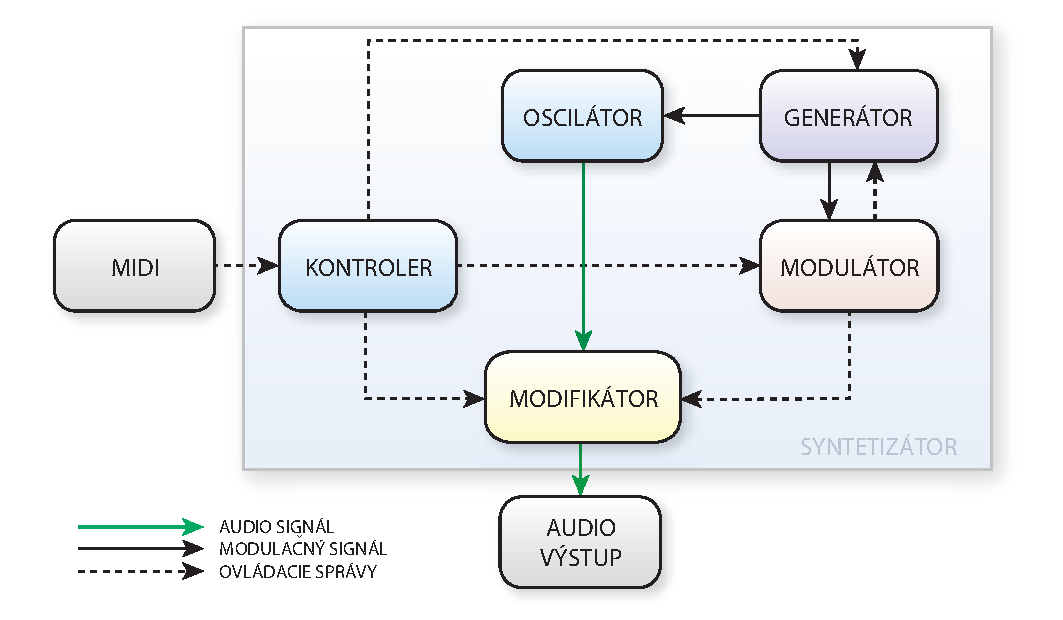
\includegraphics{obr01}}
\caption{\label{obr01} Všeobecná schéma bežného syntetizátora}
\end{figure}

Funkcia syntetizátora spočíva v transformácii interaktívnych vstupov hudobníka a aktuálnych nastavení parametrov syntetizátora na jeden alebo viacero zvukových výstupov. Bežný syntetizátor sa skladá z niekoľkých komponentov, z ktorých každý má svoju vlastnú funkciu. Základná architektúra syntetizátora je znázornená na  obr.~\ref{obr01}. Komponent \emph{kontroler} prijíma vstupy a na ich základe posiela riadiace inštrukcie do ďalších komponentov, ktoré sa spolu podieľajú na tvorbe zvukového signálu. \emph{Generátor} je komponent, ktorý generuje určitý druh signálu. Môže to byť periodický signál použitý na generovanie samotného základu zvuku syntetizátora prostredníctvom komponentu \emph{oscilátor}, nízkofrekvenčný periodický signál alebo rôzne neperiodické signály použité ako vstupy do modulátora. \emph{Modulator} je komponent, ktorý modifikuje parametre ostatných komponentov na základe vstupných hodnôt. Jednoduchým príkladom použitia modulátora je ovládanie hlasitosti alebo frekvencie oscilátora podľa signálu generovaného v ľubovoľnom generátore. \emph{Modifikátor} je komponent, ktorý spracúva zvukový signál vygenerovaný oscilátorom, a určitým spôsobom ho modifikuje. Príkladom môže byť ľubovoľný reťazec efektov a filtrov.

\subsection{Komponenty syntetizátorov}
Najčastejšie implementované komponenty v súčasných syntetizátoroch sú:
\begin{description}
\setlength{\itemsep}{-0.5ex}

\item[Oscilátor] -- základný komponent, ktorý generuje samotný základ zvuku. Najjednoduchší oscilátor vytvára sínusový signál, ale bežné implementácie ponúkajú rôzne periodické, ale aj neperiodické priebehy. Jeho frekvencia je závislá od stlačenej noty.
\item[Filter] -- komponent, ktorý odstraňuje určité frekvencie z prichádzajúceho signálu. Najčastejšie sa používajú rezonančné filtre typu low-pass (dolnopriepustný), high-pass (hornopriepustný), band-pass (prepúšťajúci určité pásmo) a band-stop\footnote{Pri niektorých syntetizátoroch uvádzaný ako BAND-REJECT alebo NOTCH filter.} (filtrujúci určité pásmo). Aktívna frekvencia (Hraničná pre low-pass a high-pass, priepustná pre band-pass a filtrujúca pre band-stop) týchto filtrov býva ovládateľná, ako aj miera rezonancie, resp. šírka pásma.
\item[Generátor obálky] -- generuje neperiodický signál, ktorý má za úlohu najmä ohraničiť amplitúdu signálu v priebehu hrania noty. Základný princíp obálky je určiť rýchlosť rastu amplitúdy signálu pri stlačení klávesu, priebeh počas hrajúcej noty a rýchlosť klesania po pustení noty. Funkcia obálky nie je obmedzená na moduláciu amplitúdy signálu, ale môže byť implementovaná pre moduláciu ktoréhokoľvek parametera elementov syntézy.
\item[Nízkofrekvenčný oscilátor (LFO)] -- generuje nízkofrekvenčný  \newfootnote{Nízkymi frekvenciami v kontexte syntézy zvuku v hudbe rozumieme frekvencie prevažne nižšie ako počuteľné spektrum. To neznamená, že nízkofrekvenčné oscilátory nemôžu generovať počuteľné frekvencie, ale že ich primárnym cieľom nie je generovať zvuk.} signál, ktorý býva použitý na moduláciu niektorého parametra syntetizátora. Tento generátor môže mať, podobne ako zvukový oscilátor, rôzne priebehy.
\item[Modulačná matica (Modulation Matrix)] -- tabuľka zapojení modulačných zdrojov ku modulovaným parametrom.
\item[Efektová jednotka] -- komponent, ktorý na vygenerovaný signál aplikuje rôzne efekty obohacujúce zvuk. Tento komponent býva zapojený až po spojení signálov jednotlivých hlasov.



\end{description}


\subsection{Vstupy syntetizátorov}
Existujú rôzne spôsoby, akými môže hudobník so syntetizátorom interagovať. Najčastejšia forma je ovládanie prostredníctvom klaviatúry podobnej klavíru, ale nie je výnimočné ani používanie strunových senzorov pre gitary, dychové ovládače, alebo dokonca senzory pohybu. Pre jednotné rozhranie ovládania syntetizátorov, ale aj iných hudobných zariadení, a ich vzájomnú komunikáciu a interakciu bol vyvinutý štandard MIDI. Okrem MIDI inštrukcií môže syntetizátor prijímať aj audio signál a použiť ho ako modulačný vstup.

\subsection{Výstupy syntetizátorov}
Výstupom syntetizátorov je jeden alebo viacero zvukových signálov. V praxi sa bežne používa minimálne jeden stereovýstup, väčšina moderných syntetizátorov však disponuje dvoma a viacerými stereovýstupmi. Vďaka viacerým výstupom je možné zo syntetizátora súčasne nahrávať napríklad surový a efektovaný signál alebo v prípade multitimbrálnych syntetizátorov nahrávať rôzne nástroje ako samostatné stopy. 

Kvôli komunikácii s inými hudobnými zariadeniami disponujú syntetizátory aj MIDI výstupom.

\section{MIDI štandard}
\label{midi}

MIDI je štandardizované rozhranie pre komunikáciu, ovládanie a synchronizáciu elektronických hudobných nástrojov. MIDI nepracuje s audiosignálom, ale prenáša správy a inštrukcie (napríklad o tom, ktorú notu a s akou intenzitou má nástroj zahrať), ovládacie (napr. zmena parametrov) a synchronizačné signály.

\begin{figure}[ht]
\centering
\resizebox{3cm}{!}{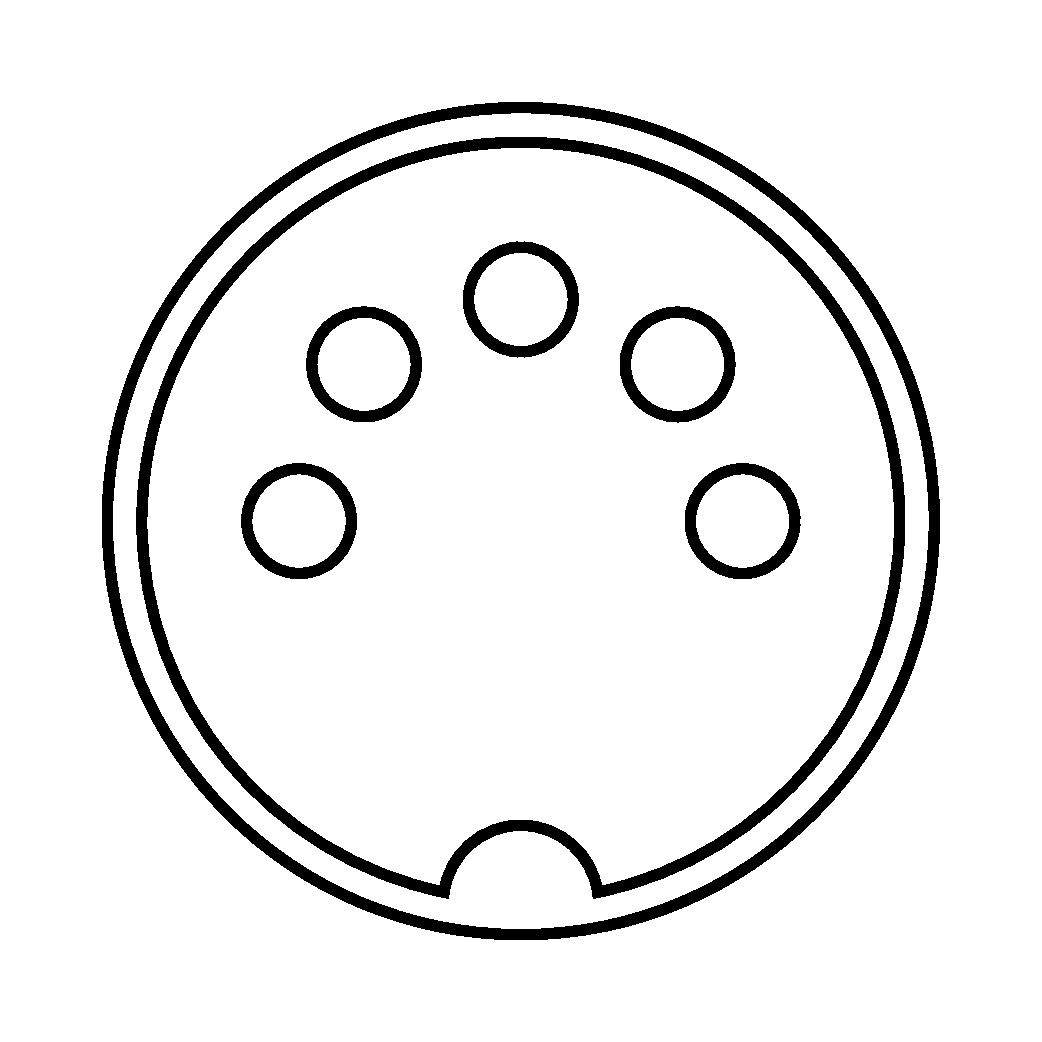
\includegraphics{midi_connector}}
\caption{\label{obr02} Štandardný konektor pre MIDI}
\end{figure}

Tento štandard bol od uvedenia v roku 1983 veľmi úspešný a všetci významní výrobcovia elektronických hudobných nástrojov ho veľmi rýchlo implementovali do svojich výrobkov. Za 25 rokov existencie sa tento štandard udržal v takmer nezmenenej podobe. Počas týchto rokov bolo viacero pokusov o modernizáciu tohto štandardu a tiež o vytvorenie nových, ako napríklad OSC\footnote{OSC - Open Sound Control.}, ale žiadny z nich nezískal dostatočnú pozornosť na to, aby nahradil štandard MIDI.

\subsection{Architektúra MIDI}
MIDI zariadenia sa podľa pôvodného návrhu zapájajú sériovo. Takmer každé MIDI zariadenie disponuje konektorom THRU, ktorý vlastne len posiela ďalej signál zo vstupu. MIDI rozhranie ponúka 16 kanálov, ktoré zdieľajú šírku pásma 30,5 kb/s.  Teoreticky nie je obmedzené, koľko zariadení je možné takýmto spôsobom zapojiť, avšak každé zariadenie vysiela prijaté dáta ďalej s určitým oneskorením a aj šírka pásma, ktorá pri tomto starom rozhraní je na dnešné pomery veľmi úzka, sa pri dlhšom zreťazení rýchlo zahltí. Preto sa v dnešnej dobe, keď už existuju rôzne MIDI smerovače, odporúča zapájať len jedno zariadenie na každú vetvu. Nástroje, ktoré využívajú vysokú multitimbraritu (zvukové moduly, samplery), disponujú viacerými MIDI vstupmi/výstupmi.

\subsection{MIDI správy}
MIDI protokol je založený na elementárnych správach. Správa pozostáva z jedného alebo viacerých bajtov. Každá správa začína takzvaným stavovým bajtom, ktorý určuje typ správy. Tento bajt sa odlišuje od ostatných tým, že má nastavený prvý bit na hodnotu 1. Takto je možné rozoznať začiatok novej správy. Prvá polovica bajtu definuje typ správy a druhá určuje, do ktorého zo šestnástich MIDI kanálov správa patrí.

Najdôležitejšie typy správ a im prislúchajúce hodnoty sú:

\begin{description}
\setlength{\itemsep}{-0.5ex}

\item[Note Off (8)] -- zastavenie noty,
\item[Note On (9)] -- spustenie noty,
\item[Polyphonic Aftertouch (A)] -- zmena prítlaku klávesu\newfootnote{Polyfonický Aftertouch je v MIDI klávesoch veľmi zriedka implementovaný.},
\item[Control Change (B)] -- zmena hodnoty ovládača,
\item[Program Change (C)] -- zmena programu\newfootnote{Program je zoznam konkrétnych nastavení všetkých parametrov nástroja. Zmena programu teda znamená zmenu nastavení na iné nastavenia uložené v pamäti.},
\item[Aftertouch (D)] -- zmena prítlaku platná pre všetky noty v rámci kanálu,
\item[Pitch Wheel (E)] -- ovládač určený hlavne pre ohýbanie tónu.
\end{description}

Týmito správami presne určujeme syntetizátoru, čo má robiť. Prvý krok je stlačenie noty, ktoré vyšle správu stlačenia noty spolu s dvomi parametrami - ktorá nota bola stlačená a akou rýchlosťou bola stlačená. Táto rýchlosť sa označuje slovom VELOCITY. Kým je nota stlačená, zmenou prítlaku sa vysielajú hodnoty AFTERTOUCH, prípadne POLY-AFTERTOUCH. Hodnoty CONTROL CHANGE (CC) sú hodnoty ovládacích prvkov - väčšinou potenciometrov. Pri zmene konkrétneho ovládača sa vyšle správa CC s číslom ovládača a jeho hodnotou. Pri pustení klávesu sa vysiela správa NOTE OFF a rýchlosť pustenia klávesu\newfootnote{Rýchlosť pustenia klávesu tiež nie je často implementovaná v MIDI klávesoch.}.

Noty, rýchlosť stlačenia, ovládače, hodnoty ovládačov sú v rozmedzí 0 -- 127. Jednou z mála výnimiek je ovládač PITCH WHEEL, ktorý nadobúda hodnoty --8192 až +8191.

\section{Typy syntézy}

Rokmi vývoja syntetizátorov uzrelo svetlo sveta veľa rôznych typov syntézy. Od veľmi jednoduchého kombinovania niekoľkých harmonických signálov až po veľmi zložité fyzikálno-akustické simulácie. Hlavne digitálne syntetizátory priniesli obrovské množstvo nových možností.

\subsection{Aditívna syntéza}
Asi najjednoduchším používaným typom syntézy je aditívna syntéza. Už názov tejto metódy napovedá, že ide o sčítavanie určitých elementárnych signálov. Základ zvuku všetkých hudobných nástrojov je zložený zo základnej frekvencie a jej vyšších harmonických frekvencií\newfootnote{Harmonická frekvencia určitej frekvencie je jej celočíselný násobok, napríklad frekvencia 100~Hz má harmonické frekvencie 200~Hz, 300~Hz, 400~Hz,...}. Amplitúdy jednotlivých harmonických zložiek sa pri týchto nástrojoch časom menia. Na tomto princípe je založená aditívna syntéza, ktorá generuje určitý počet harmonických signálov, pričom každá z nich má vlastnú amplitúdovú obálku. Tieto obálky umožňujú meniť pomery harmonických zložiek, a tým meniť farbu zvuku.

Táto technika ponúka napríklad veľmi zaujímavé možnosti simulácie strunových nástrojov a organov. Moderné aditívne syntetizátory kombinujú aditívnu syntézu s~prvkami iných typov syntéz. Významným hardvérovým aditívnym syntetizátorom je \emph{KAWAI K5000} a zo softvéru sú to najmä \emph{VirSyn Cube} a \emph{Camel Audio Cameleon}.

\subsection{Subtraktívna syntéza}
Subtraktívna syntéza je zrejme najstarší populárny typ syntézy. Väčšina analógových syntetizátorov fungovala na tomto princípe, a preto sa digitálnym a softvérovým subtraktívnym syntetizátorom často hovorí aj \bq virtuálne analógové\eq .

Ich princíp spočíva v generovaní signálu bohatého na harmonické zložky a následnom filtrovaní rezonančnými filtrami. Väčšina subtraktívnych syntetizátorov využíva 2~alebo~3 oscilátory s voliteľnými priebehmi, medzi ktorými najčastejšie býva píla (SAWTOOTH), trojuholník (TRIANGLE) a obdĺžnik (SQUARE). Hlavne píla a obdĺžnik sú priebehy s vysokou úrovňou harmonických frekvencií a pri týchto priebehoch sa filtrovaním dosahujú špecifické zvuky. Napríklad syntetizátor \emph{Roland TB-303} sa preslávil hlavne svojím originálne znejúcim filtrom. Ďalším známym subtraktívnym nástrojom je \emph{Clavia Nord Lead}.

\subsection{Wavetable syntéza}
Wavetable syntéza je v niečom podobná aditívnej a v niečom sample-based syntéze. Využíva digitálne vzorky akustických nástrojov, lenže na rozdiel od sample-based syntézy používa len niekoľko krátkych vzoriek, väčšinou dlhých len jednu periódu základnej frekvencie. Medzi týmito vzorkami pri prehrávaní plynule prechádza z jednej do~druhej, a vytvára tak kváziperiodický signál a tým pomerne realistický zvuk. Podobnosť s aditívnou syntézou je v tom, že vzhľadom na použitie vzoriek o dĺžke rovnajúcej sa jednej perióde aj wavetable syntéza využíva len harmonické frekvencie, pretože neharmonické frekvencie nemôže takáto vzorka obsahovať. Podobný je aj spôsob plynulého prechádzania z jednej vzorky do druhej, čo vlastne produkuje podobný efekt, ako zmeny pomerov harmonických frekvencií pri aditívnej syntéze. Oproti aditívnej syntéze má ale táto metóda výhodu v tom, že vyžaduje oveľa menej výpočtov v reálnom čase. Populárnym wavetable syntetizátorom je \emph{Microwave} od firmy \emph{Waldorf}.

\subsection{FM syntéza}
V roku 1983 predstavila spoločnosť \emph{Yamaha} modely \emph{DX7} a \emph{DX9}, ktoré využívali frekvenčnú moduláciu oscilátorov ako spôsob vytvárania zvuku. Model DX7 sa stal veľmi populárnym a jeho emulácie sú dodnes používané. Niektoré FM syntetizátory používajú sínusový priebeh pre modulačný aj modulovaný signál, iné dávajú na výber z viacerých priebehov. Táto metóda umožňuje vytvárať širokú škálu zvukov. Pre vytvorenie harmonických zvukov je dôležité, aby modulačný a modulovaný signál boli vzájomne harmonické. 

\subsection{Granulárna syntéza}

Granulárna syntéza je založená na veľmi krátkych vzorkách (bežne 1 -- 50~ms) nahratého alebo syntetizovaného zvukového materiálu. Tieto vzorky sa nazývaju granule a pri prehrávaní sú navzájom vrstvené a prehrávajú sa s premenlivým vzájomným časovým posunom, premenlivou frekvenciou, fázou a amplitúdou. Týmto sa dosahujú rôzne umelé efekty a surrealistické zvuky. Táto syntéza je pomerne málo rozšírená. Využíva ju napríklad softvérový syntetizátor \emph{Buero Stelkens crusherX-Studio}.

\subsection{Formantová syntéza}

Formantová syntéza je známa najmä zo systémov syntetizujúcich reč. Funguje na báze formantov -- úzkych pásmovopriepustných filtrov. Určitý počet týchto formantov usporiadaných určitým spôsobom vo frekvenčnej doméne vytvára konkrétne hlásky podobné ľudským. A práve týmto kombinovaním a rozmiestňovaním formantov vo frekvenčnej doméne a ich posúvaním a zmenami v čase alebo v závislosti od iných faktorov je možné syntetizovať zvuky odlišné od všetkých ostatných metód. Vydarenou implementáciou tejto formy syntézy disponuje syntetizátor \emph{Yamaha FS1R}.

\subsection{Phase distortion syntéza}

Syntézu deformácie fázy predstavila v roku 1984 spoločnosť \emph{Casio} s radom syntetizátorov \emph{CZ}. Tento typ syntézy väčšinou používa ako základný priebeh sínusovú vlnu. Bežné syntetizátory sa pri konštantnej výške tónu lineárne posúvaju vo fáze prehrávanej vlny. V tomto je metóda deformácie fázy iná. Aplikuje určitú matematickú funkciu medzi čas a fázový posun na vzorku generovaného signálu. Týmto procesom vznikne iná vlna s bohatým harmonickým obsahom. Parametrizácia tejto fázovej funkcie ponúka veľmi pestré možnosti tvorby atmosferických zvukov vyvíjajúcich sa v čase. Teoreticky metóda nie je obmedzená na sínus ako základný priebeh, ale použitie sínusu poskytuje oveľa viac variácií pri deformácii, ako iné priebehy známe zo subtraktívnych syntetizátorov. 

\subsection{Physical modelling syntéza}

Syntéza pomocou fyzikálneho modelu využíva určité fyzikálno-akustické modely, väčšinou hudobných nástrojov, na výpočet zvukového signálu. Takýto model môže napríklad popisovať správanie sa bubna pri údere. V takom prípade sa ako vstupné parametre môžu zobrať rýchlosť a presné miesto úderu. Nasleduje simulácia šírenia sa vĺn po dvojrozmernej membráne, ich odrazy od okrajov a prenos na valcové telo bubna a jeho rezonácia. Táto metóda dokáže verne kopírovať skutočný zvuk pri jednoduchých nástrojoch, ale jej výpočtová zložitosť rastie veľmi rýchlo so snahou presnejšie modelovať daný systém. Veľmi známy nástroj využívajúci prvky tejto syntézy je \emph{Korg Prophecy}.

\subsection{Sample-based syntéza}

Syntéza, založená na prehrávaní navzorkovaných signálov, je populárna od začiatku existencie digitálnych technológií. Veľmi úspešným modelom bol v osemdesiatych rokoch \emph{E-mu Emulator}. V priebehu vývoja nástrojov s týmto typom syntézy sa začali oddeľovať takzvané \bq samplery\eq\, od syntetizátorov. Samplery boli väčšinou schopné nahrať zvuk, upraviť ho pre potreby prehrávania, poskladať z rôznych navzorkovaných signálov nástroj\newfootnote{Typickým príkladom skladania nástroja z viacerých vzoriek je nahratie akustického nástroja na rôznych výškach tónu a priradenie vzoriek jednotlivým MIDI notám.} a pri použití tieto vzorky prehrávať. Mnohé firmy ponúkali tzv. \bq samplovacie cédéčka\eq , čo boli vlastne zvukové banky pre samplery. Sample-based syntetizátory na rozdiel od samplerov využívali vzorky hlavne ako základné priebehy pre svoje oscilátory a ďalej fungovali na princípe subtraktívnej syntézy. Väčšinou nedisponovali funkciami na nahrávanie alebo editáciu vzoriek. Bolo v nich možné narábať len s pôvodnou bankou dodanou výrobcom. V dnešnej dobe nie je hranica medzi týmito dvomi typmi taká ostrá. Samplery disponujú funkciami syntetizátorov a sample-based syntetizátory ponúkajú množstvo funkcií samplerov. Tento typ syntézy je oproti ostatným jednoduchý na výpočty, a preto často disponuje vysokou polyfóniou a multitimbralitou. Napríklad model \emph{E-mu Proteus 2000} disponuje polyfóniou 128 hlasov a multitimbralitou 32 nástrojov.

\subsection{Kombinovaná syntéza}

Drvivá väčšina moderných syntetizátorov implementuje viacero typov syntézy a kombinuje ich jednotlivé prvky. Kedysi boli takéto nástroje označované ako \bq hybridné\eq , ale dnes už je výnimočné, ak syntetizátor využíva len prvky jedného typu syntézy. Napríklad dnešné subtraktívne syntetizátory ponúkajú aspoň FM moduláciu, prípadne disponujú širokou škálou rôznych typov oscilátorov aplikujúcich rôzne typy syntézy, prípadne kombinované s deformáciou fázy.